%Iniciação de pacotes e linguagens
\documentclass[12pt]{article}
\usepackage{fatec-ti}
\usepackage{url}
\def\UrlBreaks{\do\/\do-}
\usepackage{graphicx,url}
\usepackage[brazil]{babel}   
\usepackage[utf8]{inputenc}
\usepackage{longtable}
\usepackage{tabularx}
\usepackage{float}
\sloppy

%Título do TCC - Projeto Integrador - Trabalho
%As contra barras são para inserir uma segunda linha ao título
\title{Template para Desenvolvimento de Artigos\\ Template Faculdade de Tecnologia SENAC Pelotas}

%Nome do Autor e do Orientador
%No caso de trabalho de aula, o orientador deve ser desconsiderado
\author{Nome do Aluno\inst{1}, Nome do Orientador\inst{1}}

%Endereço da Faculdade
\address{Curso de NOME DO CURSO -- Faculdade de Tecnologia SENAC Pelotas\\
  Rua Gonçalves Chaves 602 -- 96015560 -- Pelotas -- RS -- Brazil
  \email{\{aluno,orientador\}@senacrs.edu.br}
}

\begin{document} 

\maketitle
%Resumo em inglês - ABASTRACT (não devendo ultrapassar 10 linhas)
\begin{abstract}
  This meta-paper describes the style to be used in the manufacture of articles and abstracts of articles for publication in the proceedings / repositories of the TCCs, integration projects and articles / papers FATEC. For papers in English, you should add just an abstract
  while for the papers in Portuguese, we also ask for an abstract in
  Portuguese (``resumo''). In both cases, abstracts should not have more than
  10 lines and must be in the first page of the paper.
  
  \textbf{Keywords}: 5 separadas por vírgula.
\end{abstract}
%Resumo em Português - RESUMO (não devendo ultrapassar 10 linhas)     
\begin{resumo} 
  Este meta-artigo descreve o estilo a ser usado na confecção de artigos e
  resumos de artigos para publicação nos anais/repositórios dos TCCs, Projetos Integradores e artigos/trabalhos da FATEC. É solicitada a escrita de resumo e abstract apenas para os artigos
  escritos em português. Artigos em inglês deverão apresentar apenas abstract.
  Nos dois casos, o autor deve tomar cuidado para que o resumo (e o abstract)
  não ultrapassem 10 linhas cada, sendo que ambos devem estar na primeira
  página do artigo.
  
  \textbf{Palavras-Chave}: 5 separadas por vírgula.
\end{resumo}

%Seções...
% As seções quando criadas, automaticamente seguem uma sequência numérica, mesmo caso para as sub-seções
\section{Introdução} 

A introdução deve contemplar uma ideia sucinta do conjunto do projeto e deve ser o cartão de apresentação do projeto de forma a instigar o interesse do leitor.

Deve também apresentar a justificativa do projeto.

Ainda, pode apresentar o objetivo geral e específicos do projeto.

O sugerido é entre 1 e 2 páginas.


\section{Referencial Teórico}

O Referencial teórico deve apresentar o estado da arte do projeto. Este deve ser embasado por referências.

Aqui o autor irá escrever sobre a área em que o projeto está atuando, de forma que fique claro a viabilidade do projeto.

É recomendada a escrita de no mínimo uma página.

\subsection{Trabalhos Relacionados}

Como uma subseção de Referencial Teórico o autor irá escrever sobre sistemas/trabalhos similares ou que serviram de inspiração para o projeto proposto.

O recomendado é que se escreva sobre dois sistemas/trabalhos relacionados.

\section{Projeto de Sistema}

Breve descrição sobre o conteúdo da seção

\subsection{Levantamento de Requisitos}

Escrever sobre as técnicas para levantamento de requisitos e sobre os requisitos funcionais e não funcionais da aplicação

\subsection{Casos de Uso}

Apresentar e comentar o diagrama de casos de uso da aplicação

\subsection{Diagrama Entididade Relacionamento}

Apresentar e comentar o diagrama ER da aplicação.

Esta seção pode ser substituída por outra diagrama, caso se aplique (Diagrama de Classes, por exemplo)

\subsection{Tecnologias do Projeto}

Escrever sobre as tecnologias que foram utilizadas no projeto.

\section{Colocar aqui o nome do Sistema}

Iniciar a seção apresentando o diferencial do sistema proposto com relação aos relacionados apresentados anteriormente.

Em seguida, apresentar as principais telas do sistema e suas funcionalidades.

\section{Considerações Finais}

Apresentar aqui as conclusões, respondendo aos objetivos específicos levantados anteriormente.

\subsection{Trabalhos Futuros}

Escrever sobre funcionalidades que poderão ser desenvolvidadas futuramente para que o trabalho fique mais robusto.

\subsection{Dificuldades Encontradas}

Escrever aqui sobre as dificuldades encontradas durante a execução do projeto. Pontos que possam contribuir com pessoas que façam trabalhos relacionados ao seu.

\bibliographystyle{fatecbib}
\bibliography{fatec-ti}

\section{Informações Gerais para a escrita do artigo}

Os trabalhos devem respeitar os números de páginas impostos pelo tipo de trabalho. TCCs devem ter no máximo \textbf{12 a 20} páginas, Projeto Integrador deve conter \textbf{8 a 12} páginas e artigos solicitados como trabalhos de aula devem ir de acordo com a solicitação do Professor.

\subsection{Entregas dos Artigos}

Como este template pode ser empregado para diversos fins, as entregas são variadas, ou seja, como um trabalho de aula, o Prof. solicitante informará como deverão efetuar a entrega, no caso de um Projeto Integrador, o artigo deverá estar na Wiki de forma atualizada e ser entregue 3 cópias impressas ao Prof. da disciplina. Como trabalho de TCC, deverá ser entregue 3 cópias impressas ao Prof. da disciplina nas datas informadas.

\subsection{Figuras e Subtítulos}\label{sec:figs}


Figuras e subtítulos de tabelas deverão ser mostrados de forma centralizada a menos de uma linha da imagem ou da tabela referenciada, conforme o exemplo
(Figura~\ref{fig:exampleFig1}), outro modo de representar é conforme a Figura~\ref{fig:exampleFig2}, onde o subtítulo estoura o tamanho de uma frase apenas e deve ser justificado, muito utilizado em explicações de imagens junto da mesma. O subtítulo deve estar com fonteHelvetica, tamanho 10 e em negrito.

%Exemplo de utilização de figuras
\begin{figure}[ht]
\centering
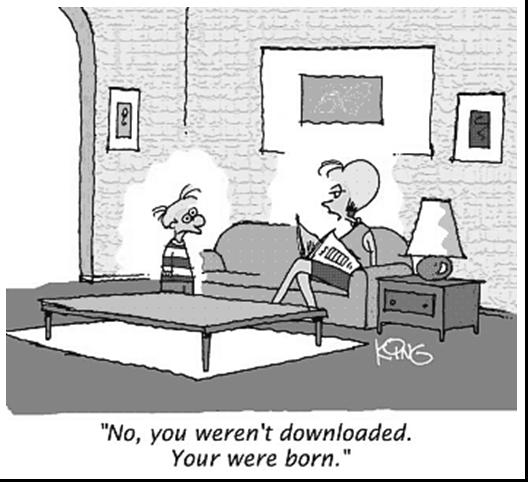
\includegraphics[width=.5\textwidth]{fig1.jpg}
\caption{Um exemplo de figura}
\label{fig:exampleFig1}
\end{figure}

\begin{figure}[ht]
\centering
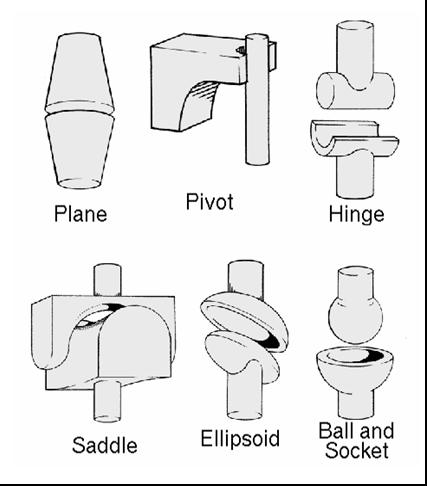
\includegraphics[width=.3\textwidth]{fig2.jpg}
\caption{Esta figura é um exemplo de figura com subtítulo explicativo que extrapolou o tamanho e deve ser justificado. Aqui passou o tamanho de uma linha.}
\label{fig:exampleFig2}
\end{figure}

Nas tabelas, o melhor é tentar evitar o uso de fundos coloridos ou sombreados, conforme evitar bordas grossas ou linhas de enquadramento desnecessários. 
As legendas das tabelas devem ser colocadas antes da tabela (ver Tabela \ref{Exemplo de Tabela})
e a fonte utilizada deve ser Helvetica, tamanho 10 e em negrito

%Exemplo de utilização de tabela
\begin{table}[!ht]
\centering
\caption{Exemplo de Tabela}
\begin{tabular}{l|c|c|c}

\hline\noalign{\smallskip}

Dificuldade			& TCC & Projeto Integrador & Trabalhos\\
\noalign{\smallskip}
\hline
\noalign{\smallskip}
Extremamente Fácil	 & X & X & X\\
Fácil	             & X & X & X\\
Médio			     & X & X & X\\
Difícil				 & X & X & X\\
Extremamente Difícil & X & X & X\\
\hline
\end{tabular}
\label{Exemplo de Tabela}
\end{table}

%Tratamento de Imagens
\subsection{Imagens}

Todas as imagens e ilustrações devem ser em tons de preto e branco, ou cinza. A resolução da imagem deve ser de cerca de 600 dpi para
imagens em preto-e-branco e 150-300 dpi para imagens em tons de cinza. Não inclua imagens com resolução excessiva, pois eles podem levar horas para imprimir, sem qualquer diferença visível no resultado.


%Referências
\subsection{Referências e Citações}

Segundo \cite{WinNT}, as referências bibliográficas devem ser inequívocas e uniformes.É recomendado dar as referências nomes de autores entre colchetes, por exemplo \cite{knuth:84}, \cite{boulic:91}, e \cite{smith:99}.

As referências devem ser listadas usando o tamanho da fonte 12. A primeira linha de cada referência não deve ser recuada, enquanto a posterior deve ser recuada em 0,5 centímetros.

As citações diretas, que indicam que estamos citando tal qual o autor disse, quando contiver menos do que 3 linhas, apenas se cita o autor colocando o seu texto entre aspas duplas. Um exemplo:

Segundo \cite{knuth:84}, "Java é a melhor do que o PHP porque diversos motivos e paga um salário mais atraente"

A citação longa é a que ultrapassa as 3 linhas, e tem uma formatação diferente, como o exemplo a seguir.

Segundo \cite{knuth:84},

\hfill
\begin{minipage}{10cm}
{\small

Java é uma linguagem de programação orientada a objetos desenvolvida na década de 90 por uma equipe de programadores chefiada por James Gosling, na empresa Sun Microsystems. Diferente das linguagens de programação convencionais, que são compiladas para código nativo, a linguagem Java é compilada para um bytecode que é interpretado por uma máquina virtual (Java Virtual Machine, mais conhecida pela sua abreviação JVM). A linguagem de programação Java é a linguagem convencional da Plataforma Java, mas não é a sua única linguagem.
\par}
\end{minipage}

\end{document}